\section{Conversione dei segnali}

    Abbiamo visto come sono fatti i dati; i dati devono essere trasformati in segnali, e questi segnali vanno trasmessi. Quando i dati devono essere trasmessi su un mezzo trasmissivo, devono essere prima convertiti.
    
    Il tipo di segnale (analogico/digitale) dipende dal mezzo trasmissivo. I tipi di dati (analogico/digitale) dipende da tutt'altri parametri.
    
    Ricordiamo che una rete di comunicazione è progettata per spedire dati da un punto all'altro. I dati devono essere convertiti in segnali analogici o digitali, e sono poi trasportati dal mezzo trasmissivo.
    
    Se la forma originale dei dati è diversa dal tipo di segnale supportato dal canale trasmissivo, può essere necessaria una conversione "dati-segnali".
    
    \begin{itemize}
        \item Analogico - Digitale
        \item Digitale - Analogico
        \item Analogico - Analogico
        \item Digitale - Digitale
    \end{itemize}
    
    Le necessità di convertire i primi due set è ovvia. Tuttavia, anche quando i dati sono nella stessa forma del segnale trasportabile può essere necessaria una conversione. 
    
    I dati digitali possono essere rappresentati in vari modi da un segnale digitale (codifica di linea); analogamente, un segnale analogico può dover essere modulato su altre frequenze per essere trasmesso su un canale analogico.
    
    \subsection{Conversione digitale-digitale}
    
        Partendo da dati digitale, li si vuole convertire in segnali digitali -- lo si fa perché i mezzi trasmissivi adoperati impongono questo tipo di rappresentazione.
        
        Può risultare ambigua la necessità di dover convertire un dato digitale in un segnale digitale. Questo succede perché l'unità di base dei dati digitali è il bit, nettamente diverso dall'unità di base dei segnali digitali, che sono elementi di voltaggi (voltaggi positivi, nulli, negativi). Si parte dunque dal presupposto che le informazioni siano salvate come bit.
        
        Si parla quindi di una rappresentazione di dati digitali usando segnali digitali. Esistono due grandi categorie di codifica (cioè conversione) digitale-digitale: la codifica di linea e la codifica a blocchi.
    
        \subsubsection{Codifiche di linea}
        
            La \textbf{codifica di linea} assume che i dati siano memorizzati nella memoria del computer come sequenze di bit. La codifica in sé permette di convertire una sequenza di bit in segnali digitali. Il mittente esegue la conversione binaria dei dati, e il destinatario ricrea i dati digitali dal segnale digitale.
            
            In questa tecnica risultano necessari un codificatore e un decodificatore. Inoltre, è possibile caratterizzarla come segue:
            
            \begin{itemize}
                \item \textbf{Unità di base dei dati e dei segnali.} Si distinguono gli elementi dei dati, intesi come i bit, e gli elementi del segnale, e si valuta il loro rapporto, che corrisponde al numero di bit rappresentati da un elemento del segnale.
                \item \textbf{Velocità dei dati e velocità del segnale.} La velocità dei dati spedibili in 1s (bps), è indicata con N, e velocità degli elementi del segnale spedibili in 1s (baud), è indicata con S. La formula risultante sarà \(S=c*n*\frac{1}/r baud\).
                \item \textbf{Linea di base.} Nella codifica di un segnale digitale, il destinatario calcola in tempo reale la media della potenza del segnale che riceve (linea di base). Il segnale ricevuto viene confrontato con la linea di base per determinare il valore dell'elemento del segnale  che si deve decodifcare. Lunghe sequenze di valori uguali falsano la media.
                \item \textbf{Componenti DC.} Quando il voltaggio di un segnale è costante per un certo periodo di tempo vengono utilizzate frequenze molto basse, vicine allo zero. Risulta un problema, poiché' su alcuni collegamenti non è è possibile il passaggio di frequenze basse.
                \item \textbf{Sincronizzazione automatica.} Per interpretare correttamente la lettura del segnale da parte del destinatario, deve corrispopndere agli intervalli di tempo usati dal mittente per generare il sdegnale. I clock possono non essere perfettamente sincronizzati, quindi serve introdurre degli elementi di sincronizzazione.
            \end{itemize}
            
            Gli schemi di codifica di linea sono schemi che permettono la rappresentazione dei dati (bit) con elementi del segnale digitale. Se ne hanno diversi. I più utilizzati in letteratura sono l'\textbf{unipolare} (NRZ), il \textbf{polare} (NRZ, RZ e bifase), il \textbf{bipolare} (AMI e pseudoternaria), il \textbf{multilivello} (2B/1Q, 8B/6T, 4D-PAM5) e il \textbf{multilinea} (MLT-3). 
            
            Il problema di passare da uno schema all'altro riguarda la sincronizzazione, e cioè legato alla capacità di decodifica del messaggio da parte del destinatario, il quale riceve un segnale digitale e deve imparare a fissare un clock di sincronizzazione che gli permettere di suddividere e decodificare tale segnale digitale.
            
            \vspace{3mm}
            
            La codifica di linea è dunque definibile come la rappresentazione, intesa come anche i livelli di voltaggio (unipolare, bipolare, etc) e come vengono organizzati, che andiamo ad utilizzare per dare informazioni di sincronizzazione.
        
        \subsubsection{Codifica NRZ}
        
            In uno schema unipolare, che è il più semplice, i valori di tutti i livelli del segnale che vengono utilizzati hanno lo stesso segno (tutti positivi o nulli, tutti negativi o nulli), e viene detto \textbf{Non-Return-to-Zero} (NRZ). 1 rappresenta un voltaggio positivo, 0 un voltaggio zero.
            
            Nell'esempio seguente, si è scelto di rappresentare il bit 1 con voltaggio positivo, e il bit 0 con voltaggio negativo.
            
            \begin{center}
                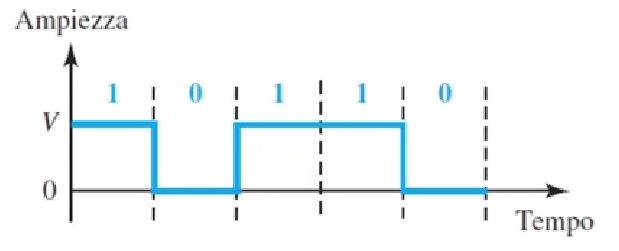
\includegraphics[scale=0.5]{images/NRZ.png}
            \end{center}
            
            Lo schema NRZ è stato poi esteso negli schemi polari per dare più informazioni sull'andamento del segnale, e cioè sulla variabilità del segnale rispetto alla rappresentazione.
            
            \vspace{3mm}
            
            Nel NRZ-L (Level), il livello del voltaggio determina il valore dei bit.
            
            Nel NRZ-I (Inverted), il valore dei bit è determinato dall'assenza o presenza di un cambio di livello del voltaggio.
            
            \begin{center}
                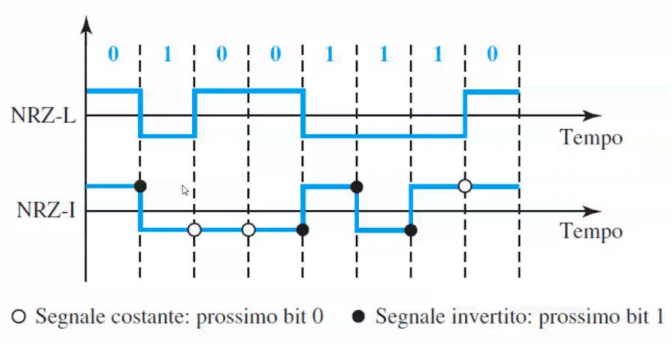
\includegraphics[scale=0.5]{images/NRZ-LeI.png}
            \end{center}
        
            Il problema principale degli schemi polari è, ad esempio, che nella codifica NRZ-L, se c'è una sequenza lunga di 0 o di 1, il valore medio della potenza del segnale si avvicinerà sempre più al valore del voltaggio positivo (o negativo) che rappresenta 0 o 1. 
            
            Il destinatario potrebbe dunque avere problemi a distinguere una tensione positiva o negativa da un'assenza di tensione. Vi è inoltre il problema della sincronizzazione dei clock fra mittente e destinatario, e dei componmenti DC. Indubbiamente, il problema più accentuato negli schema NRZ è quello della sincronizzazione.
        
        \subsubsection{Codifica RZ}
        
            La codifica RZ risolve il problema della sincronizzazione. Utilizza 3 livelli di segnale, cioè positivo, negativo e zero, e il valore 0 rappresenta una tensione negativa, mentre il valore 1 una tensione positiva. Il segnale torna sempre a zero al centro di ogni bit e rimane su tale valore fino all'inizio del prossimo bit.
            
            Nella pratica, nel RZ si parte da un elemento di segnale negativo o positivo, e si impone che si ritorni - a prescindere - sempre ad una posizione centrale, cioè nulla.
            
            \begin{center}
                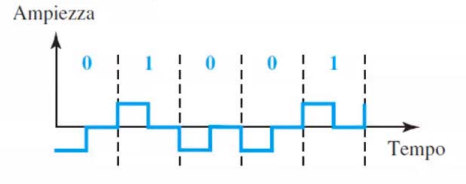
\includegraphics[scale=0.5]{images/RZ.png}
            \end{center}
        
        \subsubsection{Codifiche Manchesters}
        
            L'idea della transizione al centro di ogni bit (RZ) combinata con la codifica NRZ-L produce la codifica Manchester. Ogni singolo bit viene rappresentato da due elementi del segnale. La combinazione fra NRZ-I e RZ produce, invece, la codifica Manchester differenziale, dove ogni singolo bit viene rappresentato da due elementi del segnale.
            
            Nella codifica bifase (come le Manchesters), la transizione al centro viene usata per la sincronizzazione dei clock. La velocità richiesta è due volte quella richiesta dale codifiche NRZ.
            
            \begin{center}
                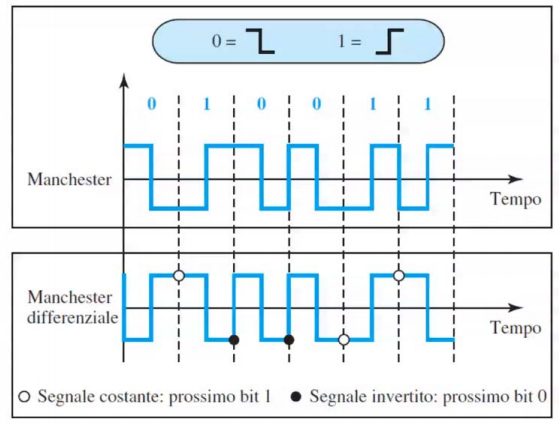
\includegraphics[scale=0.5]{images/Manchesters.png}
            \end{center}
        
        \subsubsection{Codifiche bipolari, AMI, pseudoternarie e multilivello}
        
            Nella codifica bipolare, vengono utilizzati 3 livelli del segnale: positivo, negativo e zero. Il valore di un bit viene rappresdentato o da un voltaggio pari a zero o da un voltaggio diverso da zero. Richiede la stessa velocità di segnale, ma non componenti DC. Per lunghe sequenze di 0, il vantaggio è costante. La codifica NRZ concentra la maggior parte dell'energia vicino alla frequenza nulla, e quindi non è adatta a canali che hanno cattive prestazioni per questo tipo di frequenze, mentre gli schemi bipolari concentrano l'energia attorno alla frequenza N/2.
            
            \vspace{3mm}
            
            La codifica \textbf{AMI} (Alternate Mark Inversion) rappresenta con 0 il voltaggio nullo, 1 voltaggi positivi e negativi che si alternano, ed è utilizzata per le comunicazioni a grande distanza. La codifica pseudoternaria utilizza la rappresentazione opposta.
            
            \vspace{3mm}
            
            In ogni caso, si ha la necessità di aumentare la velocità dei dati. Le codifiche multilivello hanno l'obiettivo di incrementare il numero di bit spediti in media per ogni elemento di segnale codificando una sequenza di \(m\) bit con una sequenza di n elementi del segnale. Sono solitamente indicate con sigle \(mBnL\), dove m è la lunghezza della sequenza dei dati, B indica che i dati sono binari, \(n\) è la lunghezza della sequenza del segnale, e L indica il numero di livelli.
            
            La \textbf{2B1Q} codifica 2 bit con un elemento di segnale a 4 livelli, e cioè ad una velocità doppia rispetto al NRZ-L.
        
            \subsubsection{Codifiche a blocchi}
            
                Oltre alla codifica di linea, è emersa nel tempo la codifica a blocchi. Per ottenere la sincronizzazione dei clock, occorre introdurre il concetto di ridondanza. 
                
                Se nella codifica di linea, le informazioni di sincronizzazione devono essere interpretate da come il segnale è rappresentato, nella codifica a blocchi si interviene al momento dell'invio del messaggio introducendo dei bit ridondanti, che ci permettono di capire quando terminare l'analisi di una parola.
                
                La codifica a blocchi viene solitamente chiamata codifica \(mB/nB\), perchè trasforma una parola sorgente di \(m\) bit in una parola di \(n\) bit con \(n>m\). 
                
                Ad esempio, La codifica a blocchi 4B/5B è sincronizzabile e non produce mai una sequenza con più di 3 zero consecutivi.
                
                \vspace{3mm}
                
                In genere, \textbf{vengono usate sia codifiche di linea} (per rappresentare i dati), \textbf{sia cdifiche a blocchi} (per ottenere la sincronizzazione).
            
    \subsection{Conversazione analogico-digitale}
    
        Si tratta di trasformare un dato rappresentato in forma d'onda in un segnale digitale, e cioè ad elementi del segnale. La tecnica più utilizzata per la codifica analogico-digitale prende il nome di \textit{modulazione a impulsi codificati}.
        
        \subsubsection{Modulazione a impulsi codificati}
        
            La \textbf{modulazione a impulsi codificati} converte un segnale analogico in dati digitali in tre fasi:
            
            \begin{itemize}
                \item 
                   \textbf{Campionamento.} Il segnale analogico viene campionato, e cioè misurato a intervalli regolari. Si terrà conto solo delle misurazioni fatte in questi intervalli. Il risultato sarà un numero di valori discreti.
                   
                   Il segnale analogico viene misurato a intervalli regolari $T_S$ e si stabilisce che ad ogni intervallo $T_S$ il segnale debba essere misurato. La \textbf{frequenza di campionamento} è \(f_S = \frac{1}{T_S}\).
                   
                   Vi sono tre tipi di campionamento: \textbf{ideale} (gli impulsi del segnale sono misurati in istanti di tempo a distanza $T_S$), \textbf{naturale} (la misura del segnale avviene in brevi intervalli che includono l'istante di campionamento), e \textbf{a gradini} (simile alla naturale, ma il risultato della misurazione è costante). Bisogna trovare una via di mezzo fra una qualità soddisfacente del campionamento e una buona velocità di computazione (codifica). 
                   
                   Per fare questo, si usa un risultato di Nyquist, chiamato il \textbf{Teorema di Campionamento}, che enuncia che la velocità di campionamento $f_S$ deve essere almeno due volte la frequenza più alta contenuta nel segnale $f$.
                   
                    \begin{center}
                        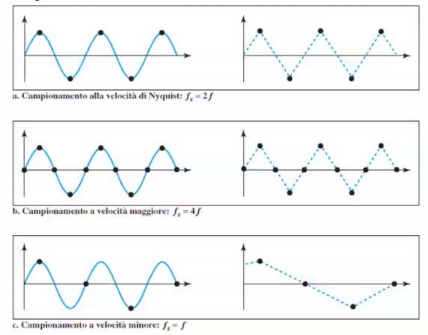
\includegraphics{images/Campionamento.png}
                    \end{center}
                
                \item
                    \textbf{Quantizzazione.} Si occupa di rappresentare le misurazioni in termini di \textit{valori}, ossia ricavare dalle misurazioni una quantificazione digitale in bit.
                    
                    Innanzitutto si individua la differenza fra l'ampieza minima e massima del segnale; dopodichè, si effettua una scelta progettuale: l'intervallo compreso fra l'ampiezza minima e massima del segnale viene diviso in $L$ intervalli d'ampiezza $\delta$. Ciascun intervallo viene rappresentato da un cosiddetto valore di quantizzazione compreso tra $0$ e $L-1$.
                
                \item
                    \textbf{Codifica.} Trasforma i valori in sequenze di bit. In particolare, si trasformano i valori di quantizzazione in sequenze di bit. Poiché i valori sono compresi fra $0$ e $L-1$, è sufficiente usare la rappresentazione binaria del valore di quantizzazione. Il numero di bit necessari è $n_b = log_2 L$.
            \end{itemize}
            
        \subsubsection{Trasmissione parallela}
                
            La conversione digitale-digitale e analogico-digitale hanno in comune la fase di codifica, ossia l'impiego di uin mezzo che richiede una rappresentazione digitale dei dati.
            
            Quando trasmettiamo su un mezzo trasmissivo dei dati digitali, si possono avere più modalità di trasmissione: trasmissione seriale e parallela. La prima usa un filo e può spedire un solo bit per volta; la seconda usa più fili e può spedire più bit alla volta.
            
            Il vantaggio della \textbf{trasmissione parallela} è la velocità di trasmissione. Lo svantaggio è il costo elevato.
            
            \vspace{3mm}
            
            Il vantaggio della \textbf{trasmissione seriale} è il costo ridotto. Lo svantaggio è costituito dalla scarsa velocità. In ogni caso, la trasmissione seriale può essere sincrona e asincrona. 
            
            \vspace{3mm}
            
            La trasmissione seriale asincrona non da molto importanza alla sincronizzazion; i bit vengono raggruppati in byte, ai quali si aggiungono informazioni intrinseche alla sincronizzazione (bit di start e bit di stop) -- è quindi un meccanismo di ridondanza. Questi bit ci permettono di dire quando inizia e finisce un byte. 
            
            \vspace{3mm}
            
            La trasmissione seriale sincrona raggruppa i flussi di bit in frame, che contiene più byte, e i bit vengono sperditi uno dopo l'altro senza bit di start e di stop, e il destinatario dovrà separare i bit dalla sequenza per ottenere i byte.
    
    \subsection{Conversione digitale-analogico}
    
        Trasforma i dati digitali in segnali analogici. \textbf{L'obiettivo è costruire un'onda analogica}, cioè un'onda sinusoidale, che è definita da ampiezza, frequenza e fase. Variando queste caratteristiche, si ottiene una differente onda e quindi dati digitali diversi. Si hanno 4 meccanismi di modulazione: ASK (\textbf{Amplitude Shift Keying}), FSK (\textbf{Frequency Shift Keying}), PSK (\textbf{Pulse Shift Keying}), QAM (\textbf{Quadrature Amplitude Modulation}). L'ultima derivate dalle prime tre.
        
        \vspace{3mm}
        
        \textbf{Dobbiamo costruire tre informazioni} (ampiezza, frequenza e fase), fissando in maniera progettuale 2 di queste dimensioni. Da queste 2, capiamo come costruire la terza. 
        
        \vspace{3mm}
        
        Nell'ASK viene modificata l'ampiezza, quindi frequenza e fase rimangono costanti. Si parla di modulazione binaria (BASK - Binary ASK), utilizza solo 2 livelli e un elemento del segnale può assumere ampiezza massima 1 e minima 0.
        
        \vspace{3mm}
        
        Nel FSK viene modificata la frequenza. Si parla di modulazione binaria (BFSK) e utilizza due frequenze portandi $f_1$ e $f_2$. $f_2$ utilizza valori 0, $f_1$ valori 1.
        
        \vspace{3mm}
        
        Nel PSK viene modificata la fase. E' la più utilizzata. Si parla di modulazione binaria (BPSK), e si hanno due tipi di segnali: uno con fase 0° e uno con fase di 180°.
        
    \subsection{Conversione analogico-analogico}
    
        Si ha necessità di fare questa conversione poiché, ad esempio, una stazione radio deve trasmettere su frequenze diverse, e cioè si ha necessità di convertire un segnale in maniera tale che possa essere trasmesso su una frequenza ammissibile rispetto al canale che stiamo utilizzando. 
        
        Si hanno 3 tecniche: AM (\textbf{Amplitude Modulation}), FM (\textbf{Frequency Modulation}) e PM (\textbf{Phase Modulation}). Concettualmente funzione come la conversione digitale-analogico: si fissano due dimensioni, se ne ricava una terza, definita dal nome della tecnica.